\begin{answer}
\begin{figure}[t] 

\centering

\subfigure[h]{

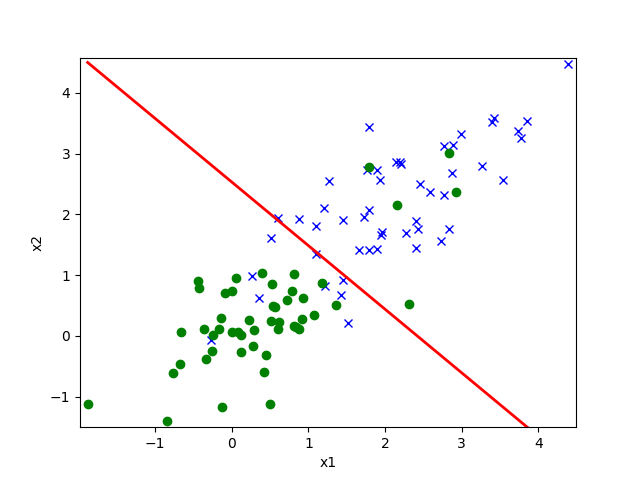
\includegraphics[width=0.35\linewidth]{tex/linearclass/logreg_pred_2.png}
\caption{Logistic Regression on Data Set 2}
}

\centering

\subfigure[h]{

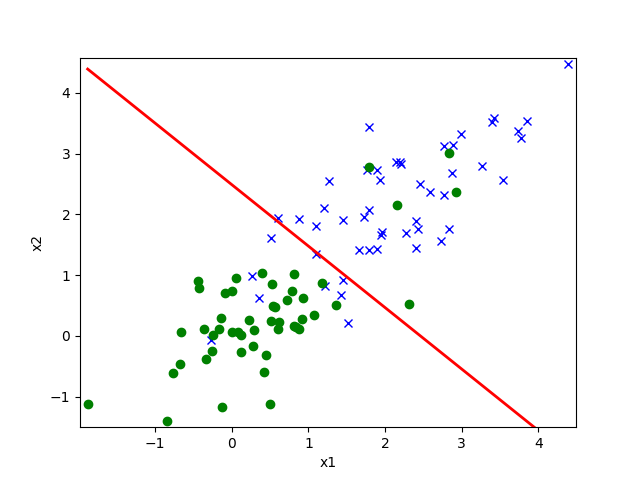
\includegraphics[width=0.35\linewidth]{tex/linearclass/gda_pred_2.png}
\caption{GDA on Data Set 2}
}
 


\label{fig:long}

\label{fig:onecol}

\end{figure}

On Data Set 1, GDA seems to perform worse than logistic regression. GDA assumes that all of the data follow Gaussian distribution. However, Data set 1 seems not to follow the Gaussian distribution so that GDA performs worse than logistic regression.

\end{answer}
